%% This is an example first chapter.  You should put chapter/appendix that you
%% write into a separate file, and add a line \include{yourfilename} to
%% main.tex, where `yourfilename.tex' is the name of the chapter/appendix file.
%% You can process specific files by typing their names in at the 
%% \files=
%% prompt when you run the file main.tex through LaTeX.
\chapter{Introduction}\label{chapter:intro}

\section{Computer Graphics state and issues}\label{intro:cg}

Computer Graphics is a vast discipline of Computer Sciences. In general, it studies theoretical methods for the synthesis of 2-dimensional (2D) images using computers. It also includes research on computer hardware, used for image computing and displaying. Among applications of computer graphics, there are typography, cinema, entertainment, scientific visualization, and industrial design. From a physical point of view, the 2D images capture information about how light beams pass through the space and reach our eyes. Then a snapshot of all received light is interpreted by our perception as a sight full of shapes and colors. 

Images in a computer are usually represented by two major archetypes. The first one is vector images \cite{aux:vector14}, which are represented by a set of 2D points, lines, polygonal shapes, and mathematically defined distribution of color within them. They are more suitable for representing schemes or text, while real-world objects would require to define hundreds of thousands of shapes to model all unique uneven patterns of materials and light. Such work is enormous in terms of computations, human hand-craft, and computer file sizes. On the other hand, raster images \cite{aux:raster94} are used. They are represented by a uniform rectangular grid (referred to as raster), filled with colored squares (referred to as pixels). Typically, colors are defined using the Red-Green-Blue (RGB) color model \cite{aux:color05}, where all possible colors are mixed from 3 primary colors, stored in computers as values in the $[0;1]$ range of real numbers (or similarly as values in $[0;255]$ range of integer numbers). Although the number of pixels may also surpass millions, the structure of pixel grids is uniform, and each pixel stores the same amount of data, allowing fast encoding and decoding in a computer. Also in most cases, the image data has information redundancy in it and thus can be compressed \cite{aux:compression18}. Besides, the pixel grid resembles a canvas from traditional art. The current computer software for the creation of raster images has capabilities similar to real brushes and palettes. This intuitive representation allows to reduce the time of image production for humans. It is known that raster images can be very realistic, proven by the visual quality that can be captured with modern digital cameras \cite{aux:camera21}.

Speaking of realism, it is one of the most important challenges in computer graphics research. The generated images should ideally be indistinguishable from the sights we perceive with our own eyes. Unfortunately, the real world is at least 3-dimensional (3D). Thus, it cannot be fully represented with images on a screen or paper, which are 2D by nature. Another obstacle is that human vision is very sensitive, and it can easily detect unrealistic or anomalous features, e.g. noise, tearing, blurriness, etc. Those are referred to as visual artifacts (also glitches, distortions). However, to this day there has not been discovered a unified metric of realism, that would allow to compare two similar images and tell which will be more plausible for the human perception \cite{metric:wang11}.

Direct usage of 2D images for visualization of the 3D world is not always efficient. For example, if we intend to create an animation (a temporarily coherent sequence of images), it would require drawing the same content with slight adjustments between images. Instead of manually copying the content from one image to another and insuring its coherency and synchronization, it is common to instead approximately model the 3D scene of interest. Such scene representations can take explicit forms, e.g. point clouds, voxel grids, triangular meshes, or even implicit functions, such as signed distance fields (SDF)\cite{survey:advances-nn22}\footnote{See Section 3.1. of \cite{survey:advances-nn22}.}\label{intro:3d-representations-paragraph}. After modeling, at every moment of time, the geometry's appearance can be projected from a certain viewpoint onto an image. This allows to model the scene one time and reuse it for the synthesis of dozens of images.

%A common way to model 3D geometry is triangular meshes \cite{mesh-data-structure}. Here the geometry is defined as a set of 3D vertices and their connectivity into polygons (usually triangles).

Typically 2D images are synthesized from a 3D scene, using rendering algorithms. They emulate the laws of physics that lie within the synthesis of images with physical cameras. One such algorithm is \textit{tracing of rays} that travel starting from a light source, and bounce from reflective surfaces, until finally, they reach an eye or a camera. This method is one of the most photo-realistic, at least to the state of our theoretical understanding of physical specular phenomena. However, it is exceptionally long to compute in great detail. That is why a much more coarse algorithm of \textit{rasterization} is typically used, with each simple geometric part of the scene (e.g. points, triangles, voxels) projected onto a 2D image. The color information for each part is extracted from texture images, that capture the physical properties of surfaces, such as color, refraction, reflection, etc (see Figure \ref{intro:fig:mesh-texture}). But with either rendering algorithm, there persists a problem that all those properties need to be explicitly specified, often by a human, which drastically increases the difficulty of achieving photo-realism. Besides, some 3D scene representations lack details, some are heavy to be efficiently processed, or require an enormous amount of computer storage. In either case, an order of magnitude higher number of geometric details needs to be defined compared to just a 2D image. 

\begin{figure}[h!]
	\centering
	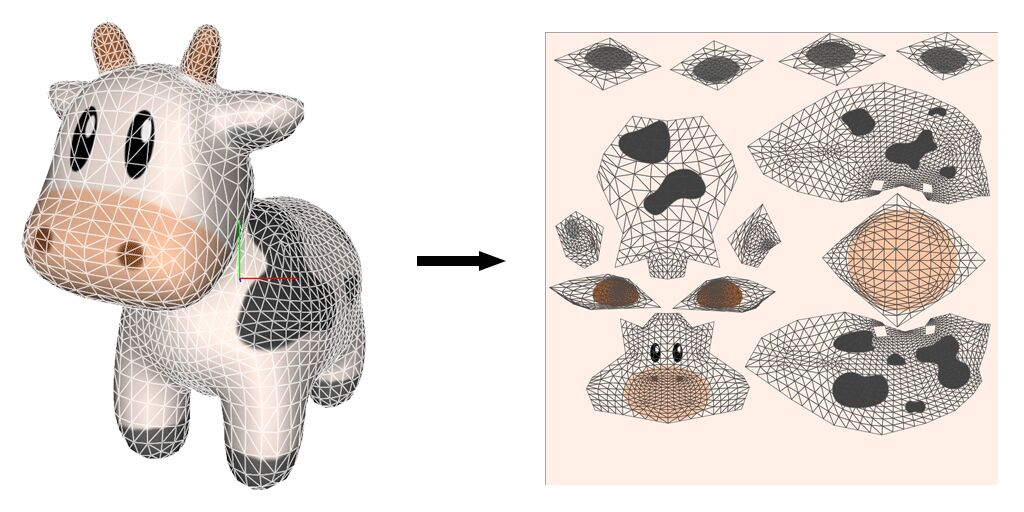
\includegraphics[height=7cm]{\imgfp/other/mesh-texture}
	\caption{Example of a triangular mesh, with a texture image wrapped on it. Each triangle is mapped to texture coordinates, which in turn allows sampling of a color patch on the texture. A rasterization process projects every triangle onto an image, and interpolates texture coordinates for every image pixel, to then sample corresponding color values from the texture. Picture source: \href{https://metalbyexample.com/textures-and-samplers/}{metalbyexample.com/textures-and-samplers}.}
	\label{intro:fig:mesh-texture}
\end{figure}


\section{Neural Rendering}\label{intro:nrender}

In the last decades, the methods of Artificial Intelligence (AI) and its sub-fields of Machine Learning (ML) and Deep Neural Networks (DNN) have emerged to solve multidisciplinary problems of science and business. Instead of modeling a phenomenon algorithmically, they aim to approximate the statistical properties of data captured from the phenomenon. Generally, input data is passed down a highly-parameterized computational graph, and output is compared to certain desired data. During a process referred to as optimization (training, tuning), the parameters of the graph are iteratively adjusted to better fit the desired data. Afterward, the computational graph is expected to be general enough to also accurately model the data, that was never seen during training. Automation is what makes these approaches groundbreaking. Unlike humans, numerical algorithms can capture very complex statistical correlations or patterns in highly-dimensional data, including images.

A selection of computer graphics problems may also be solved using ML and DNN methods. A few notable research topics in this field include:
\begin{itemize}
\item image inpainting -- the completion of missing parts on an image with semantically fitting content;
\item image super-resolution -- the up-scaling an image and making it more detailed;
\item reconstruction of 3D objects -- the automated creation of an object's 3D representation (see page \pageref{intro:3d-representations-paragraph}) and materials from 2D images captured with physical cameras;
\item neural rendering -- the automated synthesis of realistic images with the certain expected content.
\end{itemize}

This thesis focuses on the topic of neural rendering, although its definition is quite vague. A default approach is to use traditional algorithms to generate a simple image that describes coarse information about a scene, such as general outlines of each separate object, distance from a camera, etc. Then an AI model is used to generate the final image -- realistic, detailed, and possibly with higher resolution \cite{dnn:deferred19}. There is another branch of research, where the AI is used to represent the 3D scene, often implicitly as weights of the AI model. Then this representation is decoded (sampled) into 2D images using deterministic algorithms \cite{dnn:nerf20}.
 
It is very rare to have a detailed, realistic, and diverse dataset of 3D scenes that we want to reconstruct with neural rendering. Instead, AI models are typically trained on physical camera images, thus combining tasks of 3D object reconstruction and neural rendering. It is known to be a very tough challenge for man-made algorithms, and not as much easier for AI models. On the other hand, there already exist solutions that may surpass in quality the man-made image synthesis or scene modeling \cite{dnn:stylegan-v1-19,dnn:stylegan-v2-20,dnn:stylegan-v3-21,dnn:nerf20}.
 
However, training an AI model for generating photo-realistic images is only a half of the challenge. Every AI model is meant to be integrated into a real application and executed (inferred) on some computing device. It can be a stationary computer with lots of computing power. It can also be mobile hardware, since in the last years their computing power became powerful enough to infer AI models in real-time. Such hardware is included in modern smartphones, Augmented Reality (AR), or Virtual Reality (VR) head-mounted displays. Running DNN models here directly provides lower latency of computations, better privacy, and data security. But also, many performance, computational, and power usage constraints may arise:
\begin{itemize}
	\item  AI models that run in real-time applications need to deliver results multiple times per second.
	\item  The computing resources are limited due to the small physical size of the hardware. Resources are even further restricted, to reduce overheating and to improve battery life.
	\item  AI models that utilize customer devices by any means need to deal with compatibility issues (e.g. between operating systems, computing architectures, memory layouts).
\end{itemize}

This makes real usage of AI models a very challenging task. AI projects have to rely on standardized software and hardware solutions, that allow easier integration of new AI advancements. However, a unified way to efficiently run arbitrary AI models on every hardware is absent. It is often, that instead a particular AI architecture is manually integrated for a particular type of hardware, squeezing the maximum performance out of them. This is the main way out for the current projects to obtain any business value by  combining state-of-the-art hardware and AI.
 
\section{Project tasks}\label{intro:task}
 
Samsung AI Center Moscow had been researching on real-time neural rendering of human avatar images. Their recent DNN architecture \cite{dnn:stylepeople21} takes as an input a rasterized image with a body mesh with absent clothing, hair, and distinctive personal features. When trained with high image resolution, this architecture has proven to fill in those details on the image, producing good full-body (FB) images with a single person. However, the performance concerns for real-time avatar rendering were not profoundly researched.
 
%The model is trained to model appearance of a single person, captured as a 1-2 minute video from a smartphone camera. The distinctive features are learned into a neural texture, which wraps the triangular mesh, and interpretable by the DNN only to model clothes, skin, hair and facial features. 

During the summer immersion of Master's students at Skoltech in 2021, a mobile Android application project was started by the authors. It serves as a test of the performance, visual quality, and compatibility of the aforementioned neural architecture on mobile devices. The application should prepare the input data for the DNN and visualize avatar images on top of camera frames as AR, i.e. as if images are part of the captured environment. Camera movements allow observing the avatar from arbitrary distance and angle.
 
The main concern is to obtain a balance of performance and visual quality of the mobile AR application. For instance, with the minimally acceptable avatar resolution of $512\times512$ pixels, the performance of the researched DNNs is too low. Each frame computing takes more than 60 milliseconds (ms) on the most recent modern mobile hardware (Qualcomm Snapdragon 888). However, a computation time lower than 33ms per frame is required for a smooth AR experience, which is equivalent to more than 30 frames per second (FPS). Moreover, the architecture's training process could be adjusted with AR usage in mind. For example, when we move the camera close to the avatar, effectively only a small part of the body can be seen by the user. But if the DNN generates full-body images regardless, a big part of computations is wasted. And the seen part will be in a fairly low resolution. When rendered on a mobile screen with high resolution, it appears as a pixelated image in low details (see Figure \ref{intro:fig:stylepeople_frame}\protect\subref{intro:fig:stylepeople_frame:waste}). Also, the DNN should be stable in views that are possible in AR, but not present in the training data, e.g. straight top-down or bottom-up views. 

\begin{figure}[h!]
	\fboxrule=2pt
	\centering
	\begin{subfigure}[b]{0.4\textwidth}
		\centering
		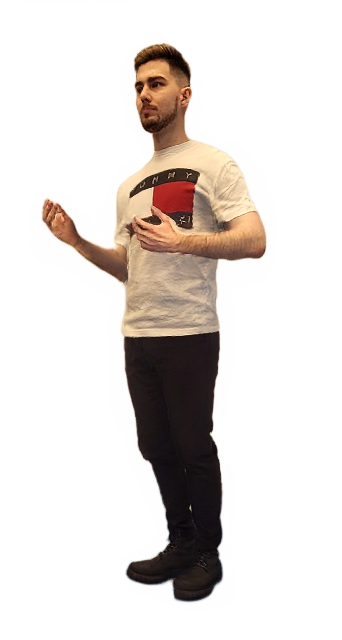
\includegraphics[height=10cm]{\imgfp/other/frame_640_narrow}
		\caption{}
		\label{intro:fig:stylepeople_frame:640}
	\end{subfigure}
	\hfill
	\begin{subfigure}[b]{0.59\textwidth}
		\centering
		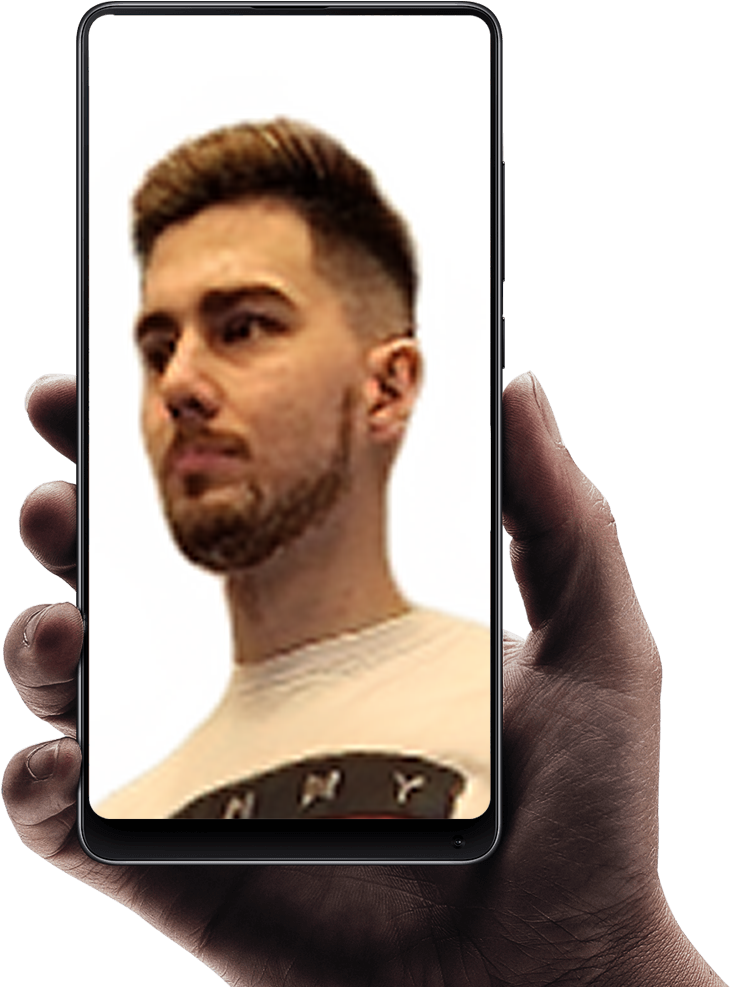
\includegraphics[height=10cm]{\imgfp/other/frame_waste}
		\caption{}
		\label{intro:fig:stylepeople_frame:waste}
	\end{subfigure}

	\caption{(\protect\subref{intro:fig:stylepeople_frame:640}) A full-body image generated with the baseline DNN \cite{dnn:stylepeople21}. (\protect\subref{intro:fig:stylepeople_frame:waste}) A full-body image synthesis for AR, but only a small image part is visible, and in low resolution, the rest is wasted.}
	\label{intro:fig:stylepeople_frame}
\end{figure}
 
The goal of this thesis is to continue the aforementioned project. The first high-level task is to achieve an admissible trade-off of performance and visual quality when executing the DNN as a part of the mobile AR experience. Target devices are the latest mobile phones running on Qualcomm Snapdragon System on the Chip (SoC), with Android operating system. The second task is to research adjustments of the DNN training to produce better quality images on zoomed scales (upper body, close-up), while retaining similar quality on the full-body scale. However, it is advisable to keep the same baseline \cite{dnn:stylepeople21} DNN architecture if possible, because the integration of a completely new pipeline may contradict the implementation of the first task, and will require significant time on obtaining better results and integration.
 
The specific tasks are defined as follows:
\begin{enumerate}
	\item To implement real-time input generation on mobile, for the baseline DNNs. This includes inference of a posed mesh of a unified human body model \cite{dnn:smplx19}, extraction of camera tracking information, mesh rasterization as a 2D image, and its passing to the DNN running on mobile.
	\item To research on decreasing inference time of the baseline \cite{dnn:stylepeople21} DNN architecture on mobile. It should be possible to infer it with real-time performance of at least 30 FPS, and resolution of the generated images above $256\times256$ pixels.
	\item To research DNN's training improvements, to make it robust to out-of-distribution views. For example, extremely far zooms, extremely close zooms, rotations, and angles of view, while preserving full-body quality.
	\item To achieve execution of the DNNs on specialized mobile hardware for fast quantized AI computations (see Section \ref{lit:mobile}). To compare the visual difference between outputs of the default model and outputs on mobile.
	\item To research algorithmic improvements that would compensate the weaknesses of plain DNN's inference, improving either performance or visual quality of avatars.

\end{enumerate}

\newpage


